% !TEX TS-program = pdflatex
% !TEX encoding = UTF-8 Unicode

% This is a simple template for a LaTeX document using the "article" class.
% See "book", "report", "letter" for other types of document.

\documentclass[11pt]{article} % use larger type; default would be 10pt

\usepackage[utf8]{inputenc} % set input encoding (not needed with XeLaTeX)

%%% Examples of Article customizations
% These packages are optional, depending whether you want the features they provide.
% See the LaTeX Companion or other references for full information.

%%% PAGE DIMENSIONS
\usepackage{geometry} % to change the page dimensions
\geometry{a4paper} % or letterpaper (US) or a5paper or....
% \geometry{margin=2in} % for example, change the margins to 2 inches all round
% \geometry{landscape} % set up the page for landscape
%   read geometry.pdf for detailed page layout information

\usepackage{graphicx} % support the \includegraphics command and options

% \usepackage[parfill]{parskip} % Activate to begin paragraphs with an empty line rather than an indent

%%% PACKAGES
\usepackage{booktabs} % for much better looking tables
\usepackage{array} % for better arrays (eg matrices) in maths
\usepackage{paralist} % very flexible & customisable lists (eg. enumerate/itemize, etc.)
\usepackage{verbatim} % adds environment for commenting out blocks of text & for better verbatim
\usepackage{subfig} % make it possible to include more than one captioned figure/table in a single float
\usepackage{graphicx}
\usepackage{float}
% These packages are all incorporated in the memoir class to one degree or another...

%%% HEADERS & FOOTERS
\usepackage{fancyhdr} % This should be set AFTER setting up the page geometry
\pagestyle{fancy} % options: empty , plain , fancy
\renewcommand{\headrulewidth}{0pt} % customise the layout...
\lhead{}\chead{}\rhead{}
\lfoot{}\cfoot{\thepage}\rfoot{}

%%% SECTION TITLE APPEARANCE
\usepackage{sectsty}
\allsectionsfont{\sffamily\mdseries\upshape} % (See the fntguide.pdf for font help)
% (This matches ConTeXt defaults)

%%% ToC (table of contents) APPEARANCE
\usepackage[nottoc,notlof,notlot]{tocbibind} % Put the bibliography in the ToC
\usepackage[titles,subfigure]{tocloft} % Alter the style of the Table of Contents
\renewcommand{\cftsecfont}{\rmfamily\mdseries\upshape}
\renewcommand{\cftsecpagefont}{\rmfamily\mdseries\upshape} % No bold!

%%% END Article customizations

%%% The "real" document content comes below...

\title{Factor Research: pb}
\author{Shiwen Lin, Pengtuan Wu}
%\date{} % Activate to display a given date or no date (if empty),
         % otherwise the current date is printed 

\begin{document}
\maketitle

\section{Data}

\subsection{Time period}
2000.1.31 – 2020.6.30. The SHARADAR data source has a fixed 20 years window. We regularly download data from there to our local in an accumulation manner so we would go beyond the 20 years limit.

\subsection{Universe}
We manually re-construct historical SP500 line-up as our universe. So this research by nature is large-cap oriented

\subsection{Data preparation}
Our fundamental analysis is based on a quarterly rebalance frequency, which also matches thel reporting period of companies. Our rebalance dates are the last dates of each quarter. Given the different earning dates of different company, at those dates, some companies latest finacial reports may have not come out yet. So directly using the rebalance date as the date for the fundamental information would cause look-forward bias. To address this, at each rebalance date, we use the most recent financial information prior to that date for each companies.

\section{Methodology}
\subsection{Z Score}
At each reabalance date, we rank the above-mentioned universe by the relevant column/factor (pb in this case). We take the z-score of the rank. We also group the universe by sector/industry to examine the z score of stocks in each group.

Note as a classical constituent of value factor, a low pb value indicates a more value-styled stock as a high pb means a more growthy stock

\subsection{IC}
We calculated the IC as the Spearman correlation between the rank of PB ratio and the forward 1 month return. We also smooth the IC series to rolling 12 month average.


\subsection{L/S Portfolio}
TBA

\section{Observation}
\subsection{Z Score}
Figure \ref{fig:pb_z_sector} shows the overview of all sectors. We break them down into the following categories:

\begin{figure}[H]
\centering
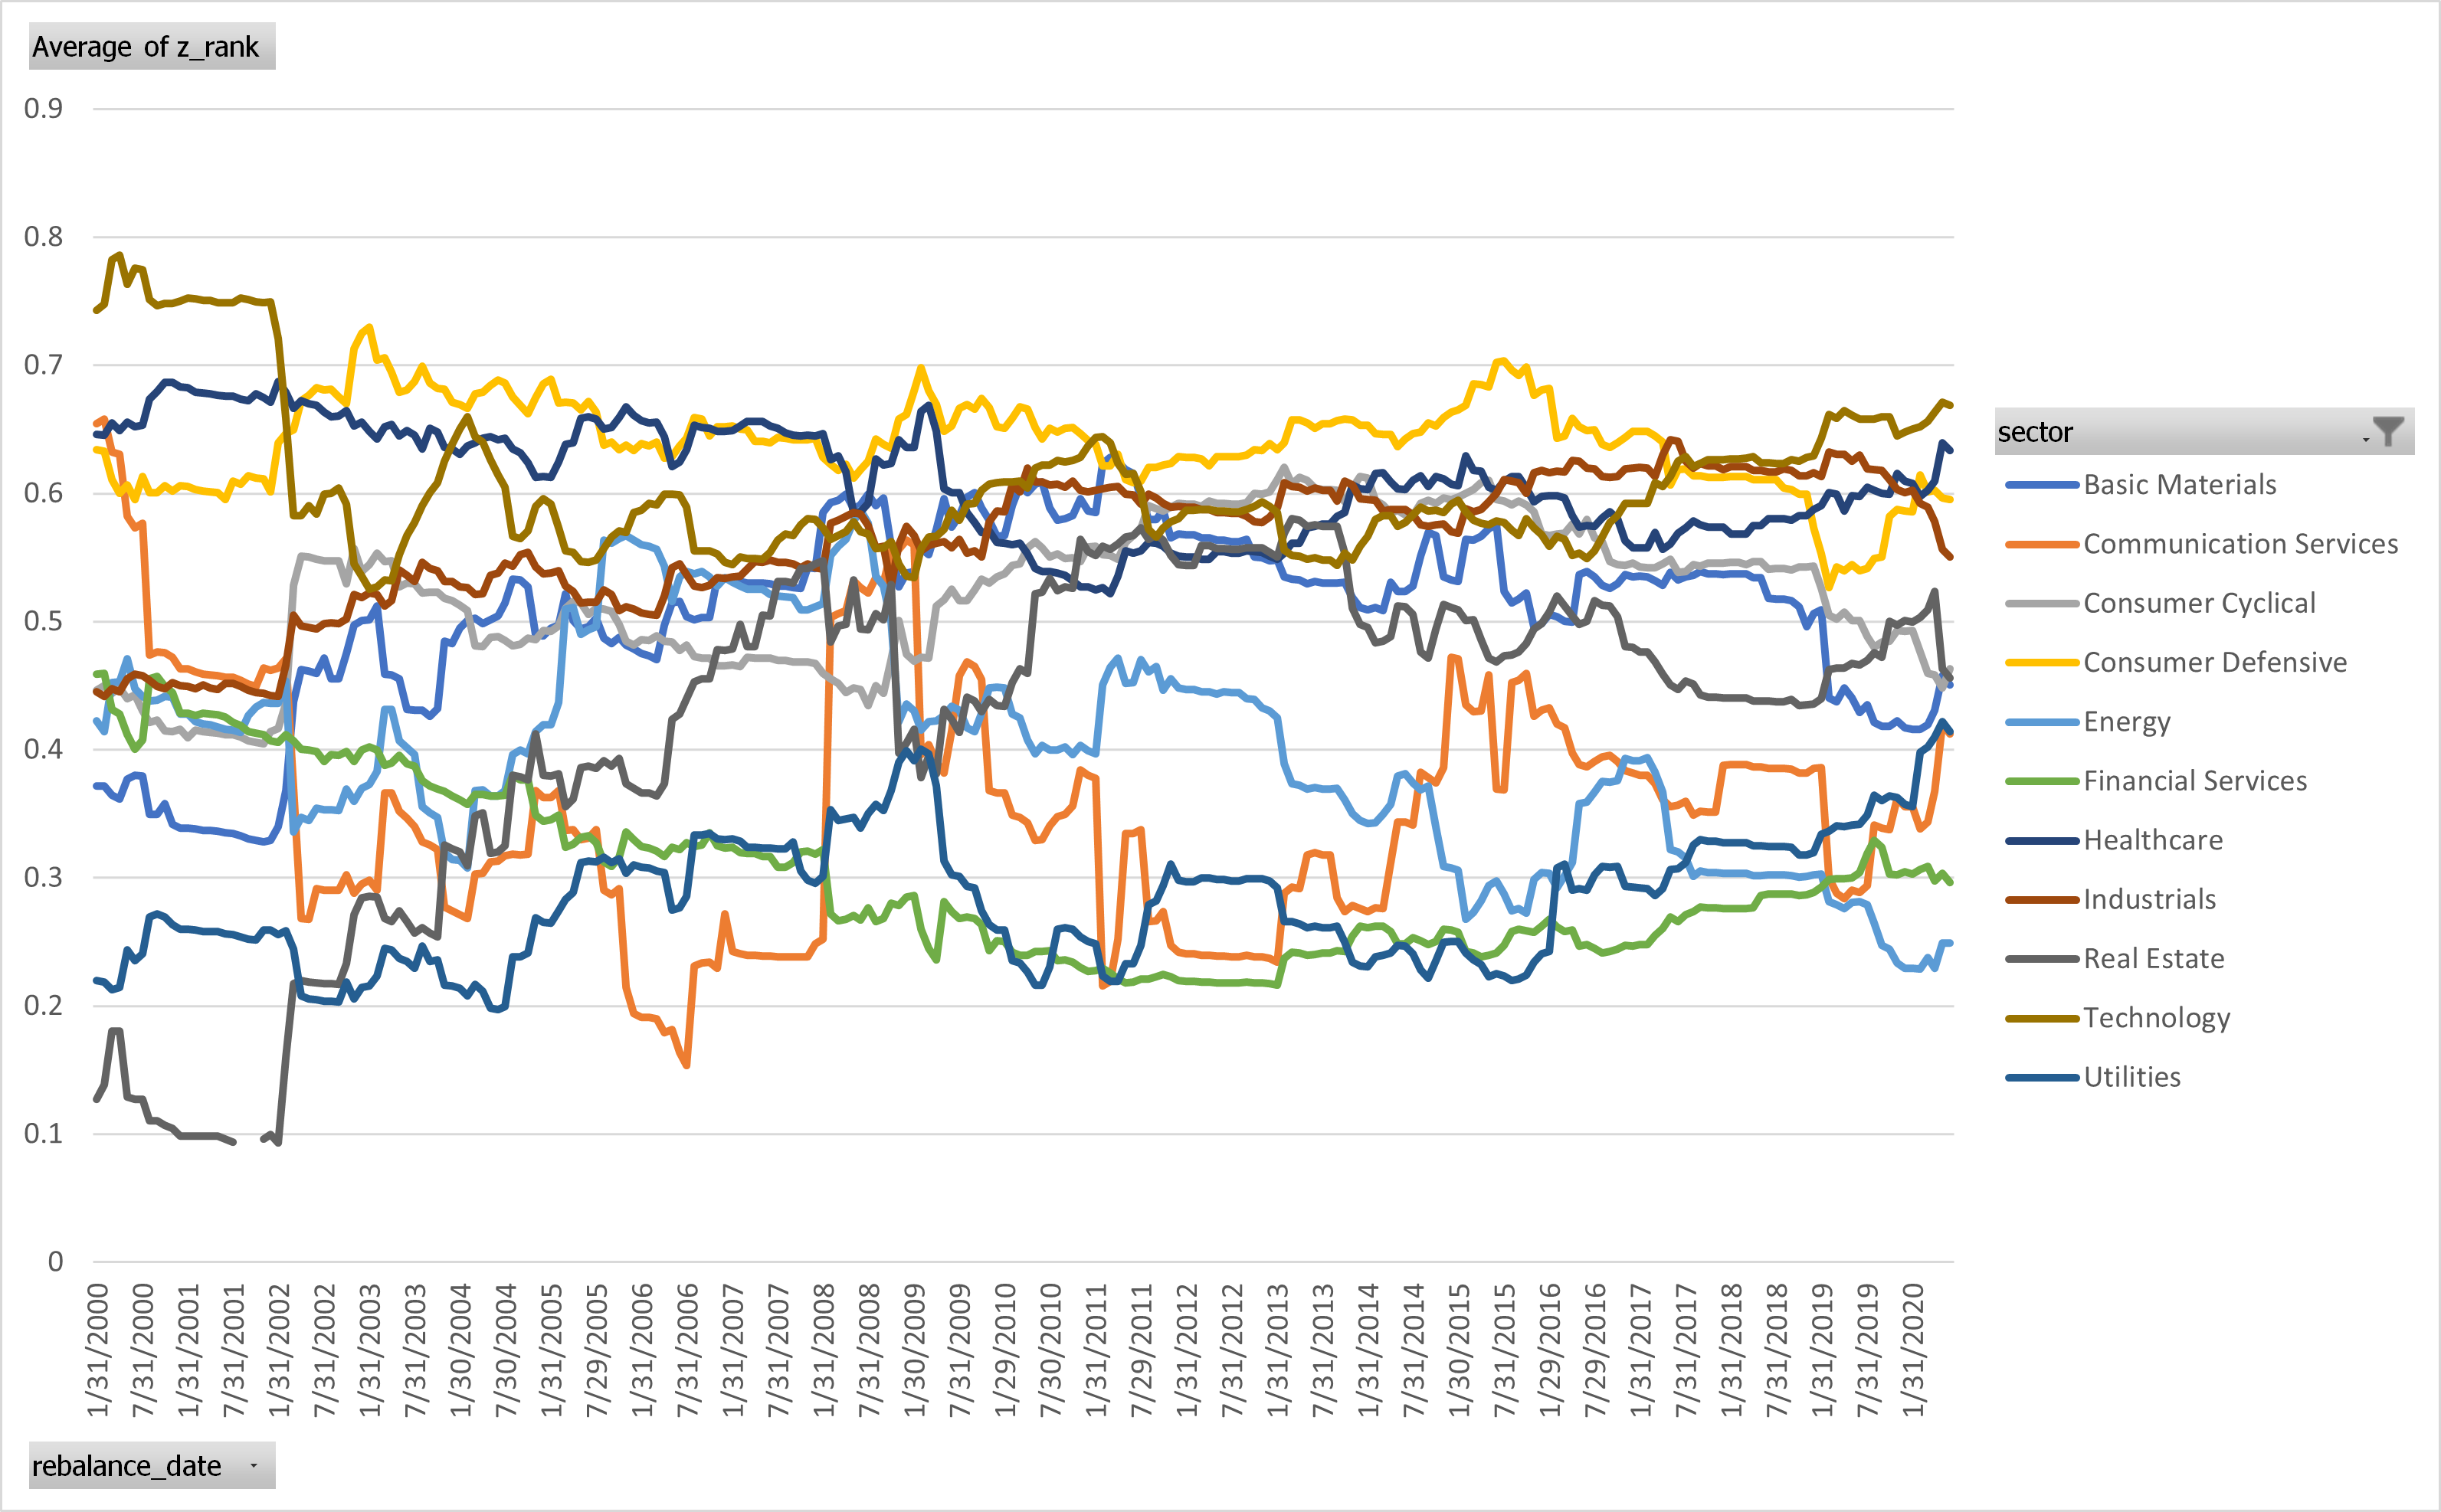
\includegraphics[scale=0.7]{pb_z_score_sector.png}
\caption{Average pb z score by each sector}
\label{fig:pb_z_sector}
\end{figure}


\begin{itemize}

\item Sectors of high z scores ($>0.5$)

As shown in Figure \ref{fig:pb_z_high}, \textbf{Technology}, \textbf{Healthcare}, \textbf{Consumer Defensive} and \textbf{Consumer Cyclical} are sectors of consistent high pb ranks historically. Among them,  \textbf{Technology}, \textbf{Healthcare} are the classical growthy sectors. For \textbf{Consumer Defensive} and \textbf{Consumer Cyclical}, we took a deeper look into the individual stocks in those sectors.

\begin{figure}[H]
\centering
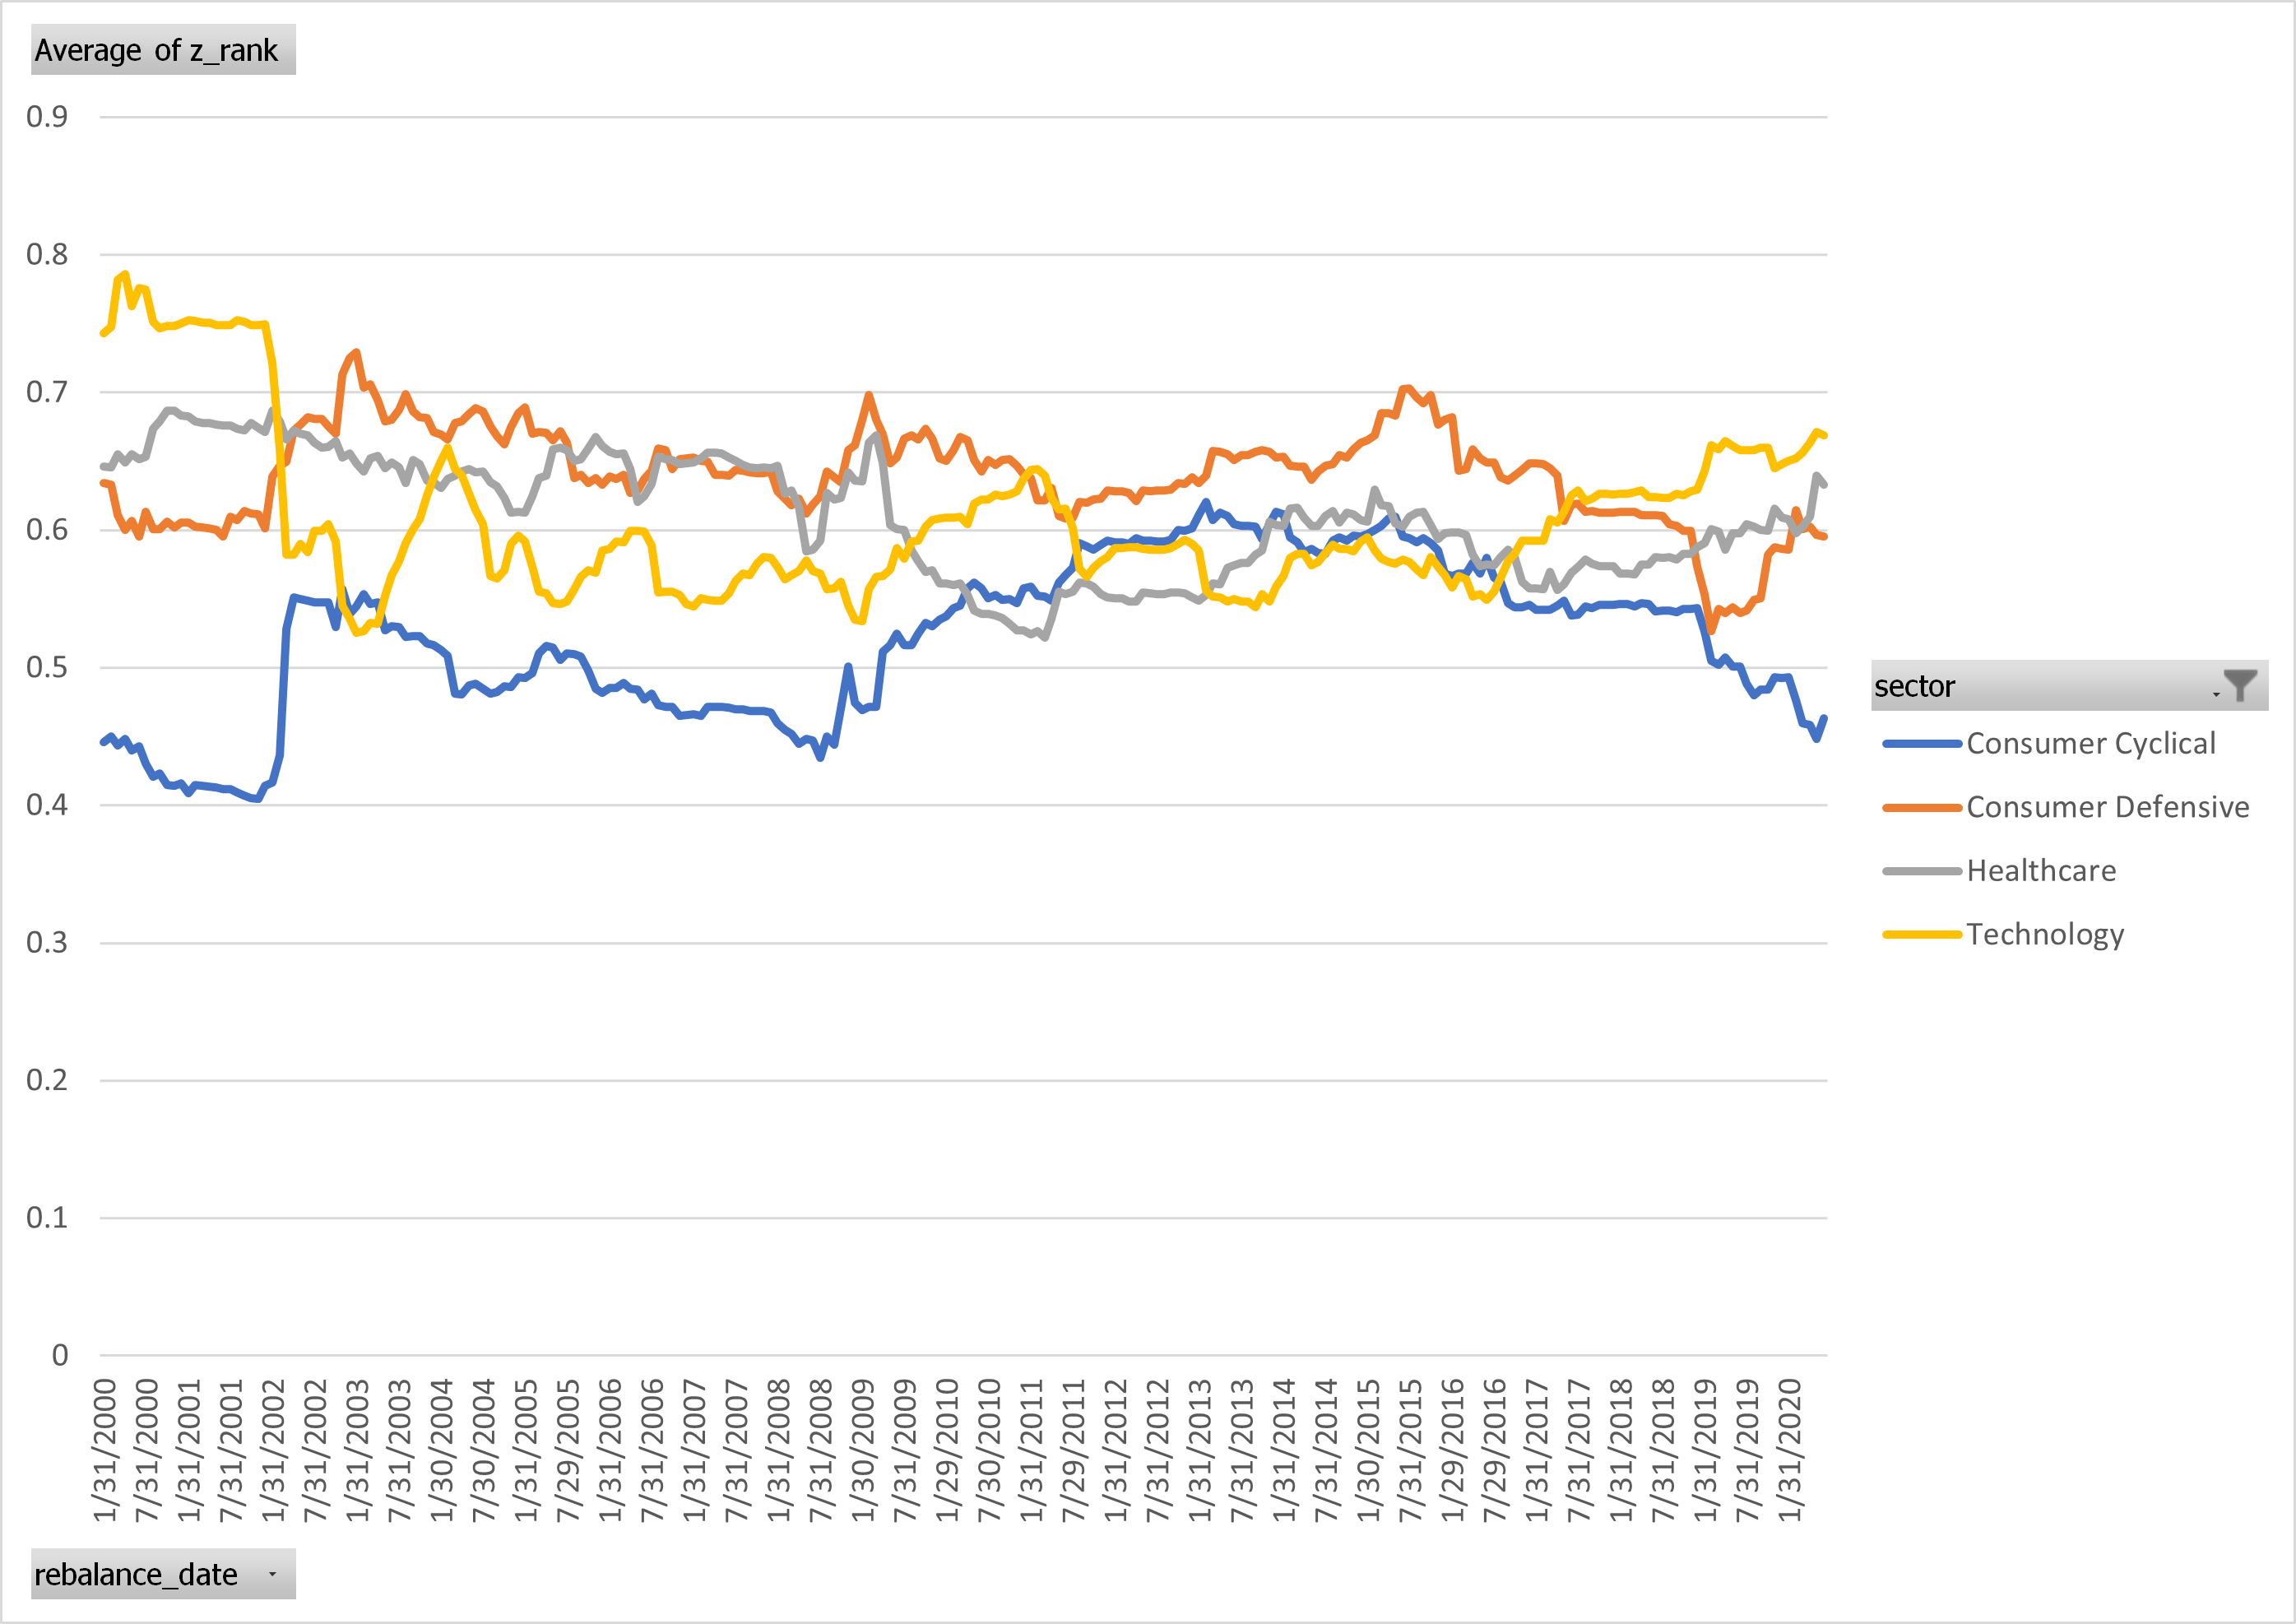
\includegraphics[scale=0.7]{pb_z_score_sector_high.png}
\caption{Sectors of high historical z-scores}
\label{fig:pb_z_high}
\end{figure}


\item Sectors of low z scores ($<0.5$)

As shown in Figure \ref{fig:pb_z_low}, \textbf{Financials } and \textbf{Utilities} have a consitent low pb rank historically. This reflects their nature as traditional value sectors.

\begin{figure}[H]
\centering
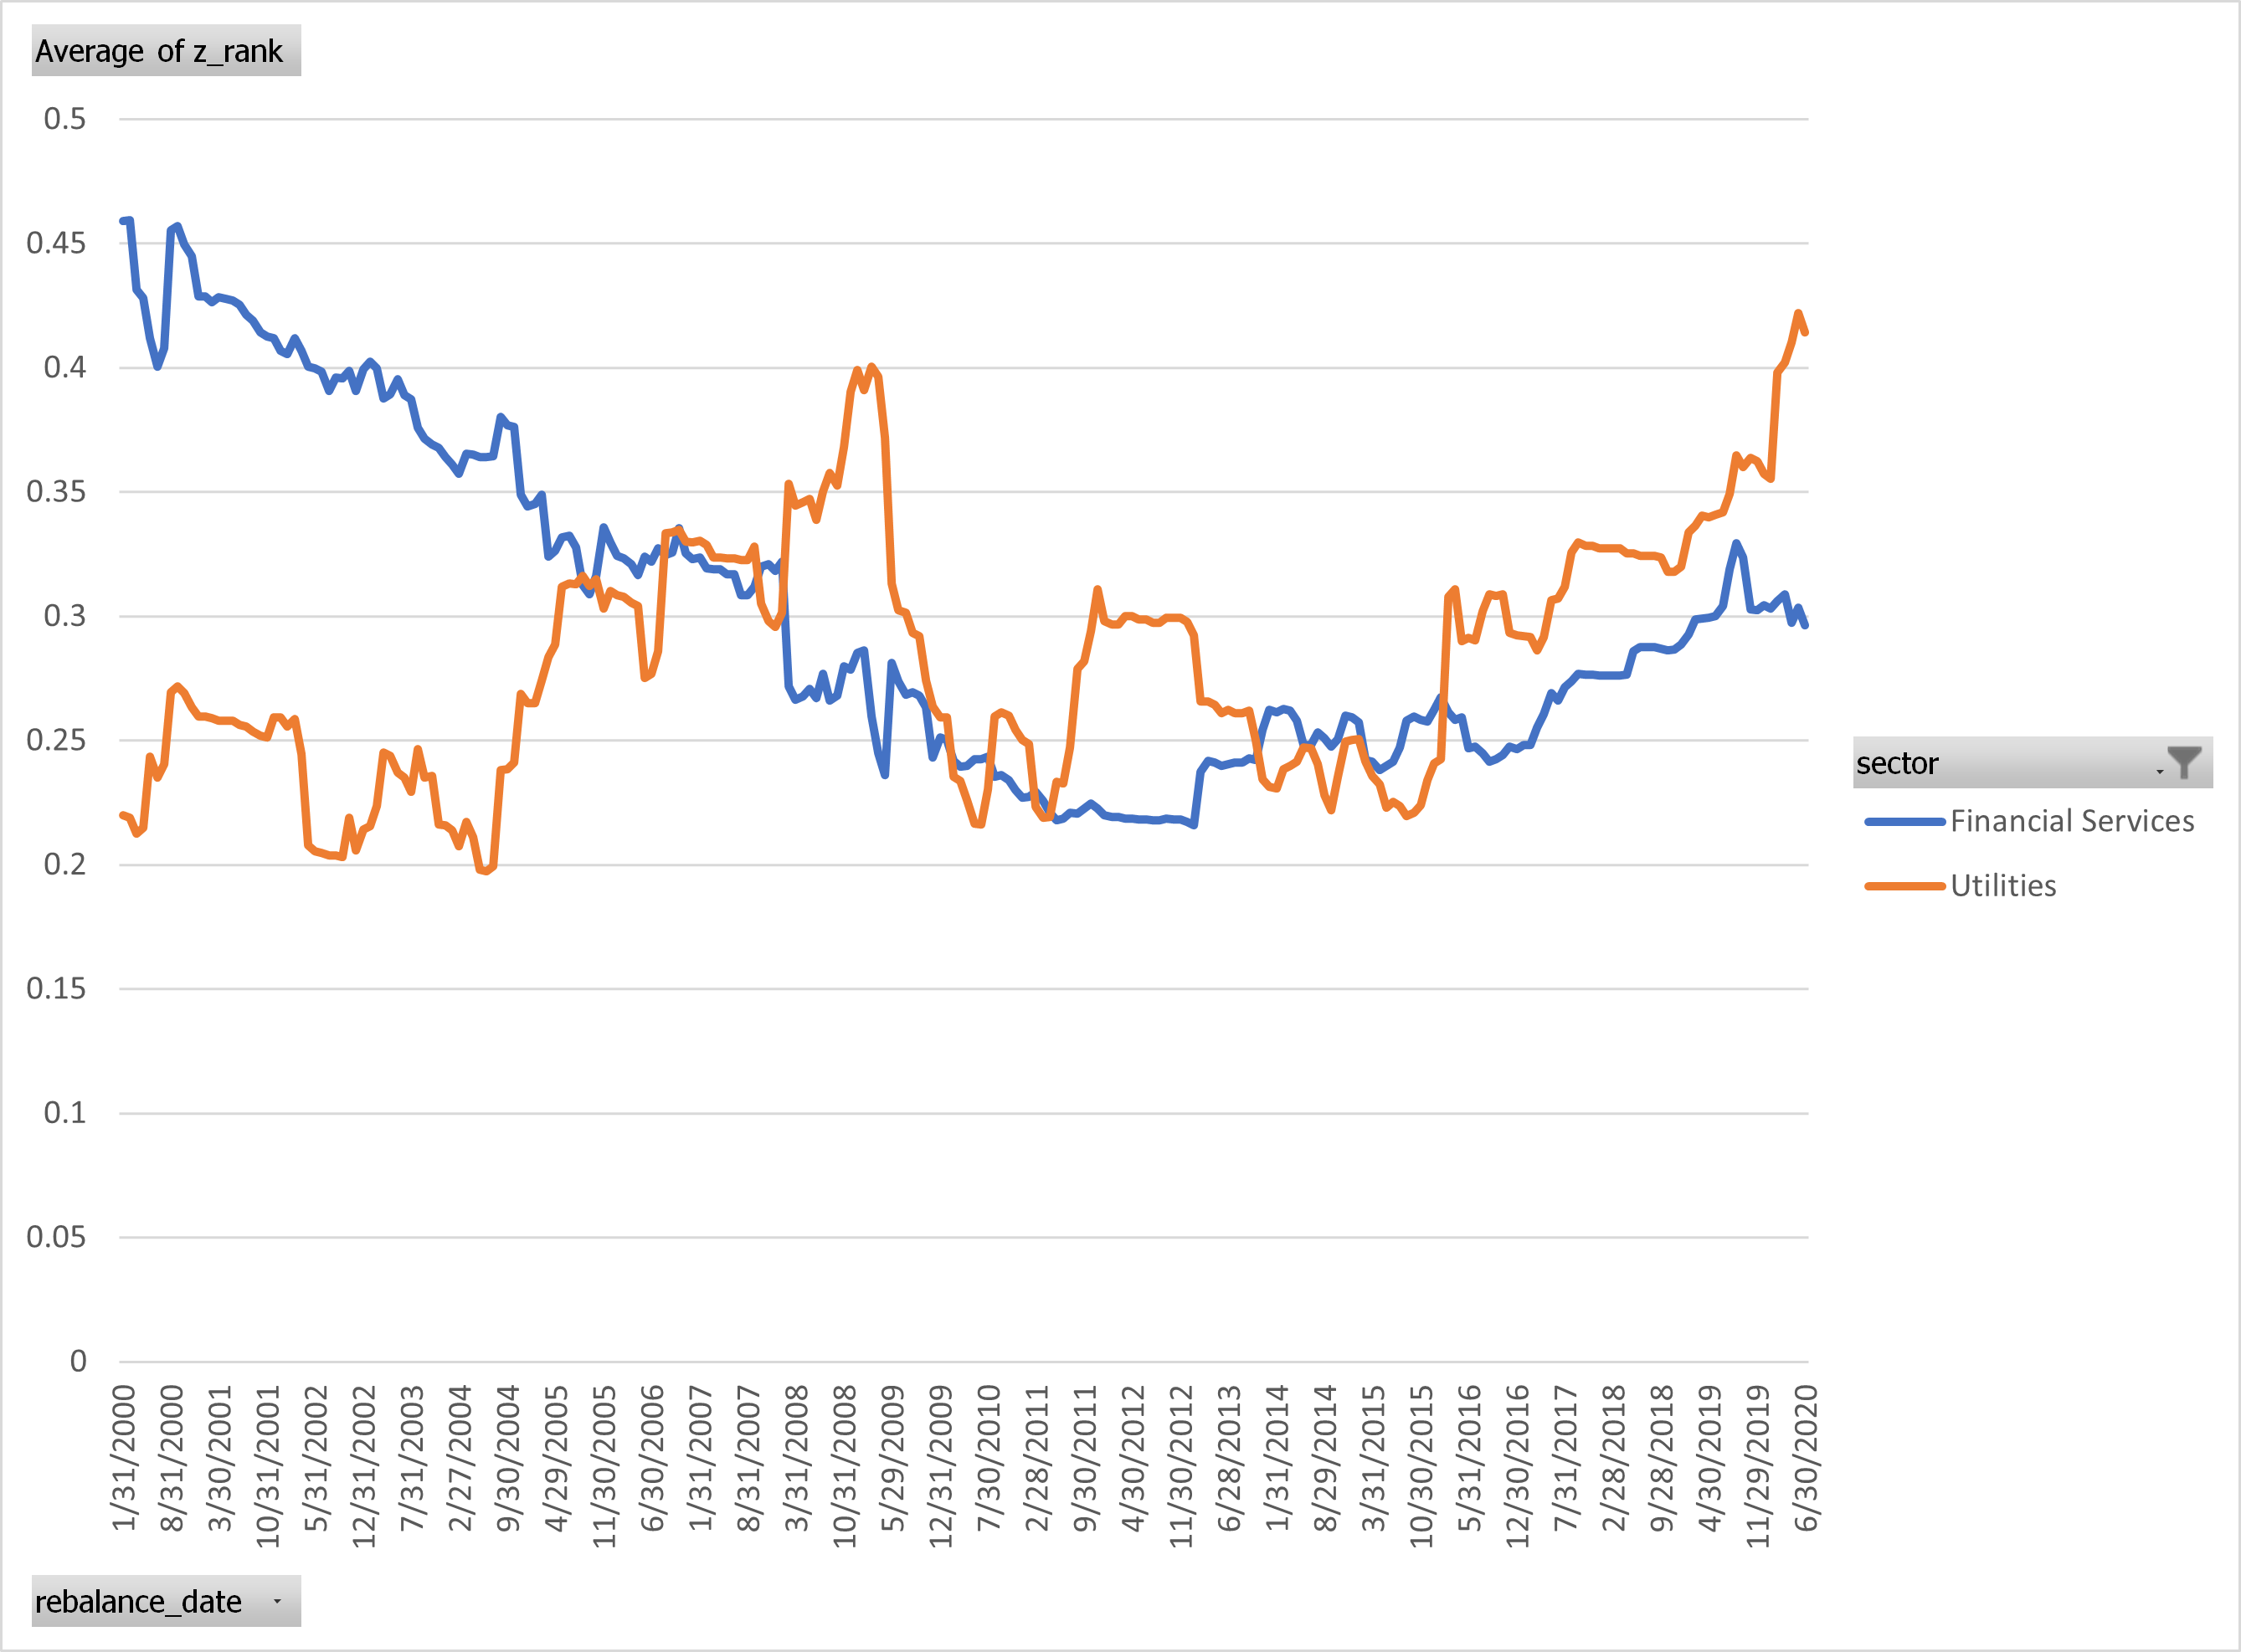
\includegraphics[scale=0.7]{pb_z_score_sector_low.png}
\caption{Sectors of low historical z-scores}
\label{fig:pb_z_low}
\end{figure}

\end{itemize}

\subsection{Sector Investigation}

\subsubsection{Consumer Defensive}
We started by looking at each industry.

\begin{figure}[H]
\centering
\includegraphics[scale=0.7]{consumer_defensive_industry.png}
\label{fig:cd_industry}
\end{figure}

The Food Distribution only has one company (in our universe) -- SYY, Sysco. As shown in Fig-\ref{fig:syy2}. This company becomes very growthy since 2019 as P/B, P/E  etc. ratios took off. Part of the reason according to Fig-\ref{fig:ssy1} is the drastic decline in its earning -- -88.1\%.However, its stock price only tank -21.3\%. This would make PE ratio relative higher than the historical average. \textbf{However, we are not able to justify its high PB ration prior to 2019}.

\begin{figure}[H]
\centering
\includegraphics[scale=0.5]{SYY2.png}
\caption{Valuations of SYY as of 9/25/2020}
\label{fig:syy2}
\end{figure}

\begin{figure}[H]
\centering
\includegraphics[scale=0.5]{SYY1.png}
\caption{Key statistics of SYY as of 9/25/2020}
\label{fig:syy1}
\end{figure}

For Beverages - Non Alcoholic sector, we took Pepsi Co (PEP) as an example. From Fig-\ref{fig:pep1} we can see that during the past one year, the valuation mesures of PEP are fairly stable. However, from Fig-\ref{fig:pep2} we observed that its Debt to Capital ratio is relatively high ~0.7x. As the book values is the net equity of the company,we wonder the high leverage causes the company's equity value relatively small and eventually leads to a higher PB ratio. We also found the similar pattern in SYY (0.8x debt ratio). \textbf{To validate our assumption that high leverage would inflate the PB ratio, we can examine the P/EV ratio which also considers companies liabilities. This would be the next topic of our factor research}.

\begin{figure}[H]
\centering
\includegraphics[scale=0.5]{PEP1.png}
\caption{Valuations of PEP as of 9/25/2020}
\label{fig:pep1}
\end{figure}

\begin{figure}[H]
\centering
\includegraphics[scale=0.5]{PEP2.png}
\caption{Key statistics of PEP as of 9/25/2020}
\label{fig:pep2}
\end{figure}


\subsubsection{Consumer Cyclical}
TBA

\subsection{IC}
From Fig \ref{fig:pb_ic_top} we observed that since the mid of 2007, pb has a positive IC ration in the majority of periods. As a hight PB means a growthy style, this exhibits a 10-year growth rally. Especially since July of 2017, high pb rank is consistently outperforming. There are some exception period where low PB outperforms buy they do not sustain. The longest period is between March 2012 to March 2013. 

We would conduct follow up research to find potential causes on what make/stop high pb working.

\begin{figure}[H]
	\centering
	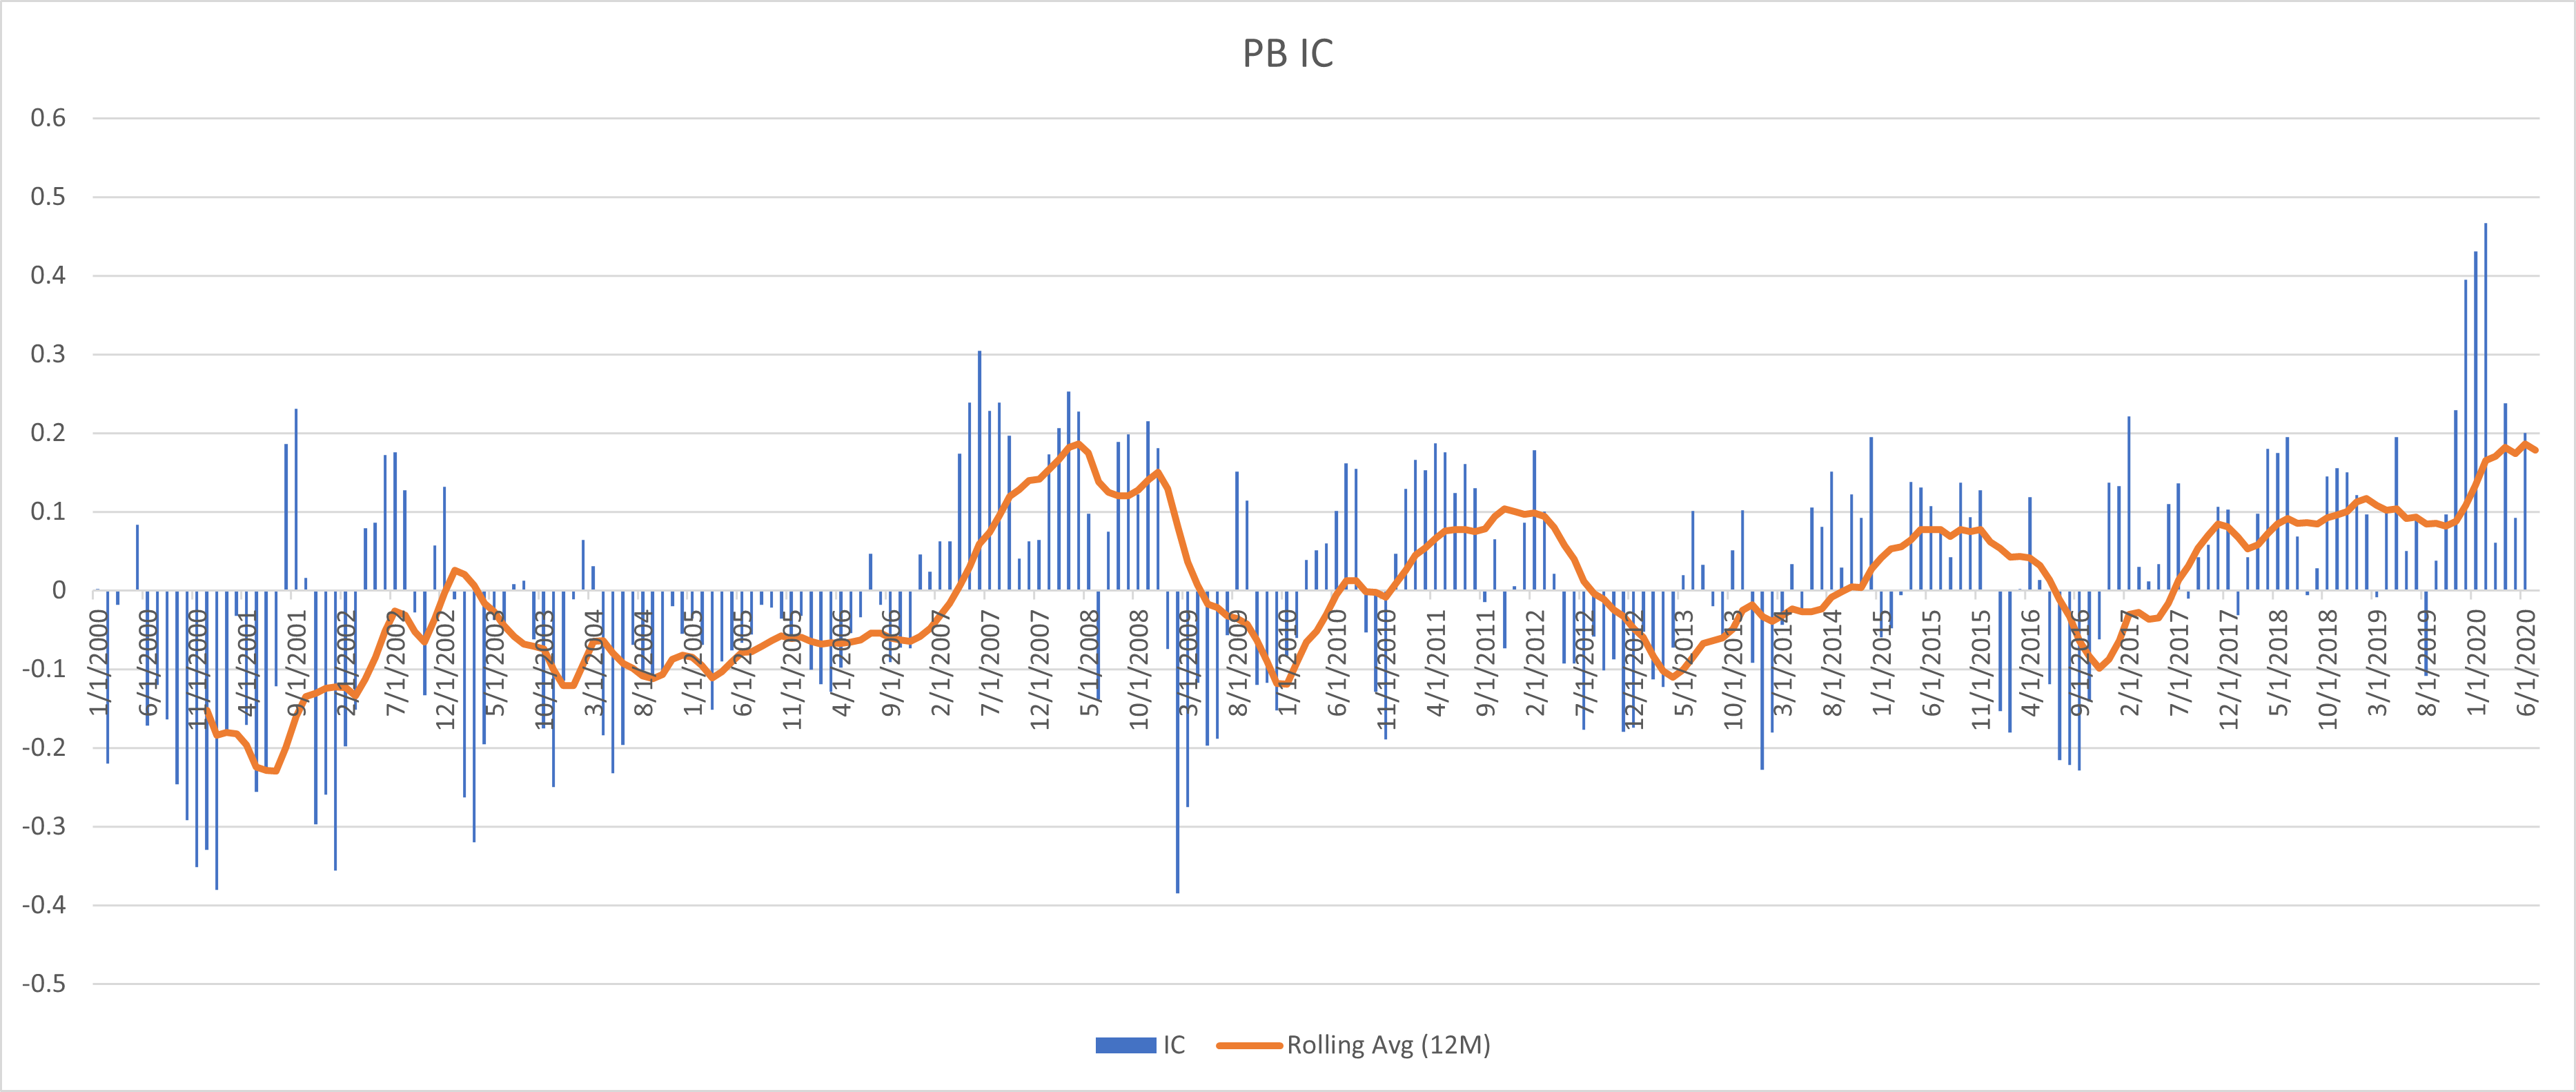
\includegraphics[scale=0.5]{pb_ic_top.png}
	\caption{Time series of IC from 2000/01/31 to 2020/07/31}
	\label{fig:pb_ic_top}
\end{figure}



\subsection{L/S Portfolio}
TBA

\end{document}
